\documentclass[11pt, twosides]{amsart}	%defines this as an article
\usepackage{chrisfriend-comp} %provides formatting declarations for page, headers, figures, textcolor, comments, and bibliographic styles
\usepackage{chrisfriend-OTF-support} %provides support for OTF system fonts; incompatible with latex, rtf2latex, & ht4latex
%\usepackage[utf8]{inputenc} %support for smallamp?

%\usepackage{tabularx}
\usepackage{tabulary} % allows for the tables I make rubrics with
%\usepackage{supertabular}
\usepackage{xtab} % allows tables to span pages
\usepackage{booktabs} % allows fancy lines in tables
%\usepackage{rotating} % allows landscape tables
\usepackage{lscape} % allows rotated longtables
\usepackage{multirow} % allows rowspanning
\usepackage{enumitem} % helps with the overview
%\usepackage{paralist}
\usepackage[nodate]{datetime} % allows the \currenttime command; nodate tells it not to mess up date settings
     \usepackage{pdflscape} % turns landscape pages sideways in PDFs; avoids kinks in neck.

%\usepackage{draftwatermark}

\usepackage{acronym}
\acrodef{ucf}[\textsc{ucf}]{the University of Central Florida}
\acrodef{dwr}[\textsc{dwr}]{the Department of Writing and Rhetoric}
\acrodef{waw}[\textsc{waw}]{Writing About Writing}
\acrodef{uwc}[\textsc{uwc}]{University Writing Center}
\acrodef{1101}[\textsc{enc~1101}]{Composition I}
\acrodef{rr}[\textsc{rr}]{Reading Response}


%%%%%%%%%% Adjust for multiple classes
\newif\ifsecondclass % Used for creating two versions of the portfolio.
% Use one of these two lines:
%\secondclasstrue 
\secondclassfalse 

% Use structure inside this comment environment to prepare multiple versions of text:
\begin{comment}
	\ifsecondclass
		This content applies to the 1130 class.
	\else % 1030 only
		This content is 1030 only.
	\fi
\end{comment}
%%%%%%%%%%%%% End multiple Versions content

\title[\textsc{enc}~1101 Syllabus]{Course Syllabus: Composition I}
\chead{\scriptsize{\fontspec[Numbers=Lining]{Garamond Premier Pro}\MakeUppercase{ENC~1101 Syllabus} }}%(Rev. \number\day\space\monthname\space\number\year)}}

  
\begin{document}
%\bibliographystyle{abbrv}

\vspace{-2in}
\begin{center}
\huge
\includegraphics[height=1.75\baselineskip]{pegasus.pdf}

\textbf{Course Syllabus: Composition I}
\end{center}


\label{sec:about_the_course}
\vspace{1.5\baselineskip}
\begin{center}
\begin{minipage}{0.76\textwidth}
%	|\hfill|
	\begin{description}[align=right, labelwidth=*, labelindent=0.9in, leftmargin=1in]
%	\item[Course Title] Composition I
	\item[Meeting]
		\ifsecondclass
		   \textsc{mwf} 11:30–12:20 (\textsc{enc} 1101.0005), \textsc{vab 217}
	\else % Full content
		\textsc{mw} 10:30–11:20 (\textsc{enc} 1101.0004), \textsc{vab 217}
	\fi
	\item[Term] Spring 2014
	\item[Instructor] Christopher R.\ Friend
	\item[Email] \href{mailto:friend@ucf.edu}{friend@ucf.edu}
	\item[Office] \href{https://www.map.ucf.edu/locations/18/colbourn-hall/}{Colbourn Hall} (\textsc{cnh}) 306\textsc{a}
	\item[Office Hours] \textsc{mw} 14:00–16:00; appointments strongly recommended. \\ Visit \href{http://friend.lattiss.com}{http://friend.lattiss.com} for availability.
\end{description}
\end{minipage}
\end{center}
\vspace{0.75\baselineskip}
\thispagestyle{empty}

%\section{Overview} % (fold)
\section{Course Description} % (fold)
\label{sub:course_description}
In this course, we will review current research on writing to learn how you and other people (students, academics, and other professionals) write in various situations. In our studies, we will focus on how:
\begin{itemize}
	\item writers and readers create meaning with texts
	\item certain writing processes and practices can be more or less effective
	\item people in different groups shape writing (and vice-versa)
	\item writing in the university is different from high school and among fields
\end{itemize}
You will use writing as a tool to help you learn each of these concepts, and you will become more aware of your style and ability as a writer. You will also learn how to examine the writing expectations in various settings, making you a more successful student and a better writer. See Table~\ref{tab:overview} for an overview of the topics studied in this course and a list of the major required papers.

% subsubsection my_version (end)
% subsection course_description (end)


% section about_the_course (end)
\section{Course Outcomes}\label{outcomes}
Through successful completion of this course and its activities, you should be able to
\begin{itemize}
	\item acquire and use strategies for reading complex, college-level texts;
	\item understand the \emph{fluid} nature of the writing process through its various components and be able to apply those components conscientiously and appropriately;
	\item use \emph{discipline-specific writing} as a means of being heard
	\item identify characteristics of a \emph{discourse community} and respond to them appropriately; and
	\item understand the concept of \emph{rhetorical situation} and be aware of its influence on your reading and writing activities, both in and out of class.
\end{itemize}

\clearpage
\section{Materials for Class}
\begin{itemize}
	\item Required
		\begin{enumerate}
\item \citeauthor{downs:2010aa}, \citetitle{downs:2010aa}, either
\begin{itemize}
	\item the brand-new \emph{Second Edition} with the white cover (\textsc{isbn} 978-1-4576-3694-3) or
	\item the \emph{First Edition} with the blue (\textsc{isbn} 978-0-312-53493-6)
\end{itemize}
		\item \citeauthor{lunsford:2010aa}, \citetitle{lunsford:2010aa}, either
		\begin{itemize}
			\item the \emph{Fifth Edition} (\textsc{isbn} 978-1-4576-6439-7) or
			\item the \emph{Fourth Edition} (\textsc{isbn} 978-0-312-66486-2)%(Bring only when requested.)
		\end{itemize}% Note: The \nameref{sec:calendar} and \href{https://webcourses.instructure.com/courses/985581/quizzes}{quizzes on Webcourses}  refer to numbering in the more widely available 4th edition. If you use the 5th edition, add one to any chapter numbers and roughly twenty-five to any page numbers in course materials.
		\item Reliable connection to the Internet. Make a plan for where you will go if your device or connection dies.
		\item Automated, reliable backup system. Every semester, I have a student who loses everything due to a hard drive failure. Don't be that student.
		\item Regular access to your \href{http://www.outlook.com/knights.ucf.edu}{Knights Mail account}. I check my account multiple times per day and will almost always reply within one business day. You should to check yours \emph{at least} once per day, but definitely before each class meeting. (Why not \href{http://www.students.graduate.ucf.edu/knights_email_for_mobile/}{set it up on your phone}?)
	\end{enumerate}
	\item Recommended
	\begin{enumerate}
		\item Google account connected to your \href{http://webcourses.instructure.com}{Webcourses} account.\footnote{You can connect the two using the \href{https://webcourses.ucf.edu/profile/settings}{Settings} link in the top-right corner of \href{http://webcourses.instructure.com}{Webcourses}.} This helps make collaboration a breeze.
		\item Dropbox account into which you store all your work. This takes care of backups.
		\item Your own computer running a full (non-mobile) operating system. Some of the work we do is much simpler with new software and the ability to run multiple programs simultaneously. Phones are too limited, and tablets can get frustrating.\footnote{Various computer labs across campus, or the loaner machines at the library, can work in a pinch.}
	\end{enumerate}
\end{itemize}

\section{Grading \& Assessment}
Your grade in this course will be based on two holistic grades listed in Table~\ref{tab:assignments}. Think of these like grades for a semester-long portfolio: the components work together to build the overall value of the whole, which will be graded in this course. You will get consistent feedback throughout the semester to help ensure you are on-track for a successful grade. Additionally, each major assignment will have a specific assessment rubric, and every smaller assignment will have detailed completion guidelines that will be provided  on \href{https://webcourses2c.instructure.com/courses/985581}{Webcourses}.  The smaller assignments are designed to help you build skills and confidence as you work toward your final project. They should not be dismissed.

Please note the following distinctive characteristics about grading in this course:
\begin{itemize}
	\item You can earn a D for an assignment or major component, but you cannot earn a D for this course. To pass, you must earn at least a C− (140 points).
	\item The grade of NC (no credit) can be assigned at the instructor’s discretion only if you complete all course work on time, participate fully, and fail to produce satisfactory work for the class.
\end{itemize}


\begin{figure}[t]
	\centering
	\subtable[Grade Calculations]{\small
		\noindent\begin{tabulary}{0.25\textwidth}{lr}
		\toprule\textbf{\textsc{Grade}} & \textbf{\textsc{Min. Points}}\\
		\midrule
			A	&	185	\\
			A−	&	180	\\
			B+	&	175	\\
			B	&	165	\\
			B−	&	160	\\
			C+	&	155	\\
			C	&	145	\\
			C−	&	140	\\
			NC	&	Unsatisfactory	\\
			F	&	Partial/Poor	\\
		\bottomrule
		\end{tabulary}\label{tab:final-grades}
	} %subtable
	\quad % Middle gap spacing
	\subtable[Grade Distribution]{\small
		\noindent\begin{tabulary}{\textwidth}{Lr}
			\toprule\textbf{\textsc{Assignment}} & \textbf{\textsc{Points}}\\
				\midrule	Product (portfolio \& other final projects)	&	100	\\
%				\midrule	Academic Research Report	&	25	\\
%				\midrule	Genre Product \& Presentation	&	25	\\
				\midrule	Process (participation \& collaboration)	&	100	\\
				\midrule	\textbf{\textsc{Total}}	& \textbf{\textsc{200}}\\
			\bottomrule
		\end{tabulary}\label{tab:assignments}
	} %subtable
	\caption{Course Grading System}
\end{figure}


\begin{table}[hb]
\caption{Assignment Overview}\label{tab:overview}
	\begin{tabulary}{\textwidth}{CLLL}
		\toprule	\textbf{\textsc{Weeks}}	&	\textbf{\textsc{Unit}}		& &	%	\textbf{\textsc{Readings}}	&	\textbf{\textsc{Minor Assignments}}	&	
		\textbf{\textsc{Major Papers}}	\\


\midrule	1	&	\multicolumn{2}{l}{\textbf{Academic Reading	}}		&		\\
\midrule	2–4	&	\multicolumn{2}{l}{\textbf{The Writing Process	}}		&	Process Analysis	\\
\midrule	5–12	&	\multicolumn{2}{l}{\textbf{Discourse Community	}}		&		\\
  	&	5	&	\emph{Concepts}	&	Characteristics Analysis	\\
  	&	6–7	&	\emph{Lexia \& Membership}	&	Definition Analysis	\\
  	&	8–9	&	\emph{Genre Awareness}	&	Genre Analysis	\\
  	&	\mbox{10–12}	&	\emph{Authority \& Identity}	&	Accommodation Analysis	\\
\midrule	13–14	&	\multicolumn{2}{l}{\textbf{Rhetorical Situations	}}		&	Rhetorical Analysis	\\
\midrule	15–16	&	\multicolumn{2}{l}{\textbf{Revision \& Reflection	}}		&	Final Portfolio	\\		
		

		\bottomrule
	\end{tabulary}
\end{table}




\begin{comment}
	\begin{figure}
		\centering	\caption{Map of Course Topics}
				 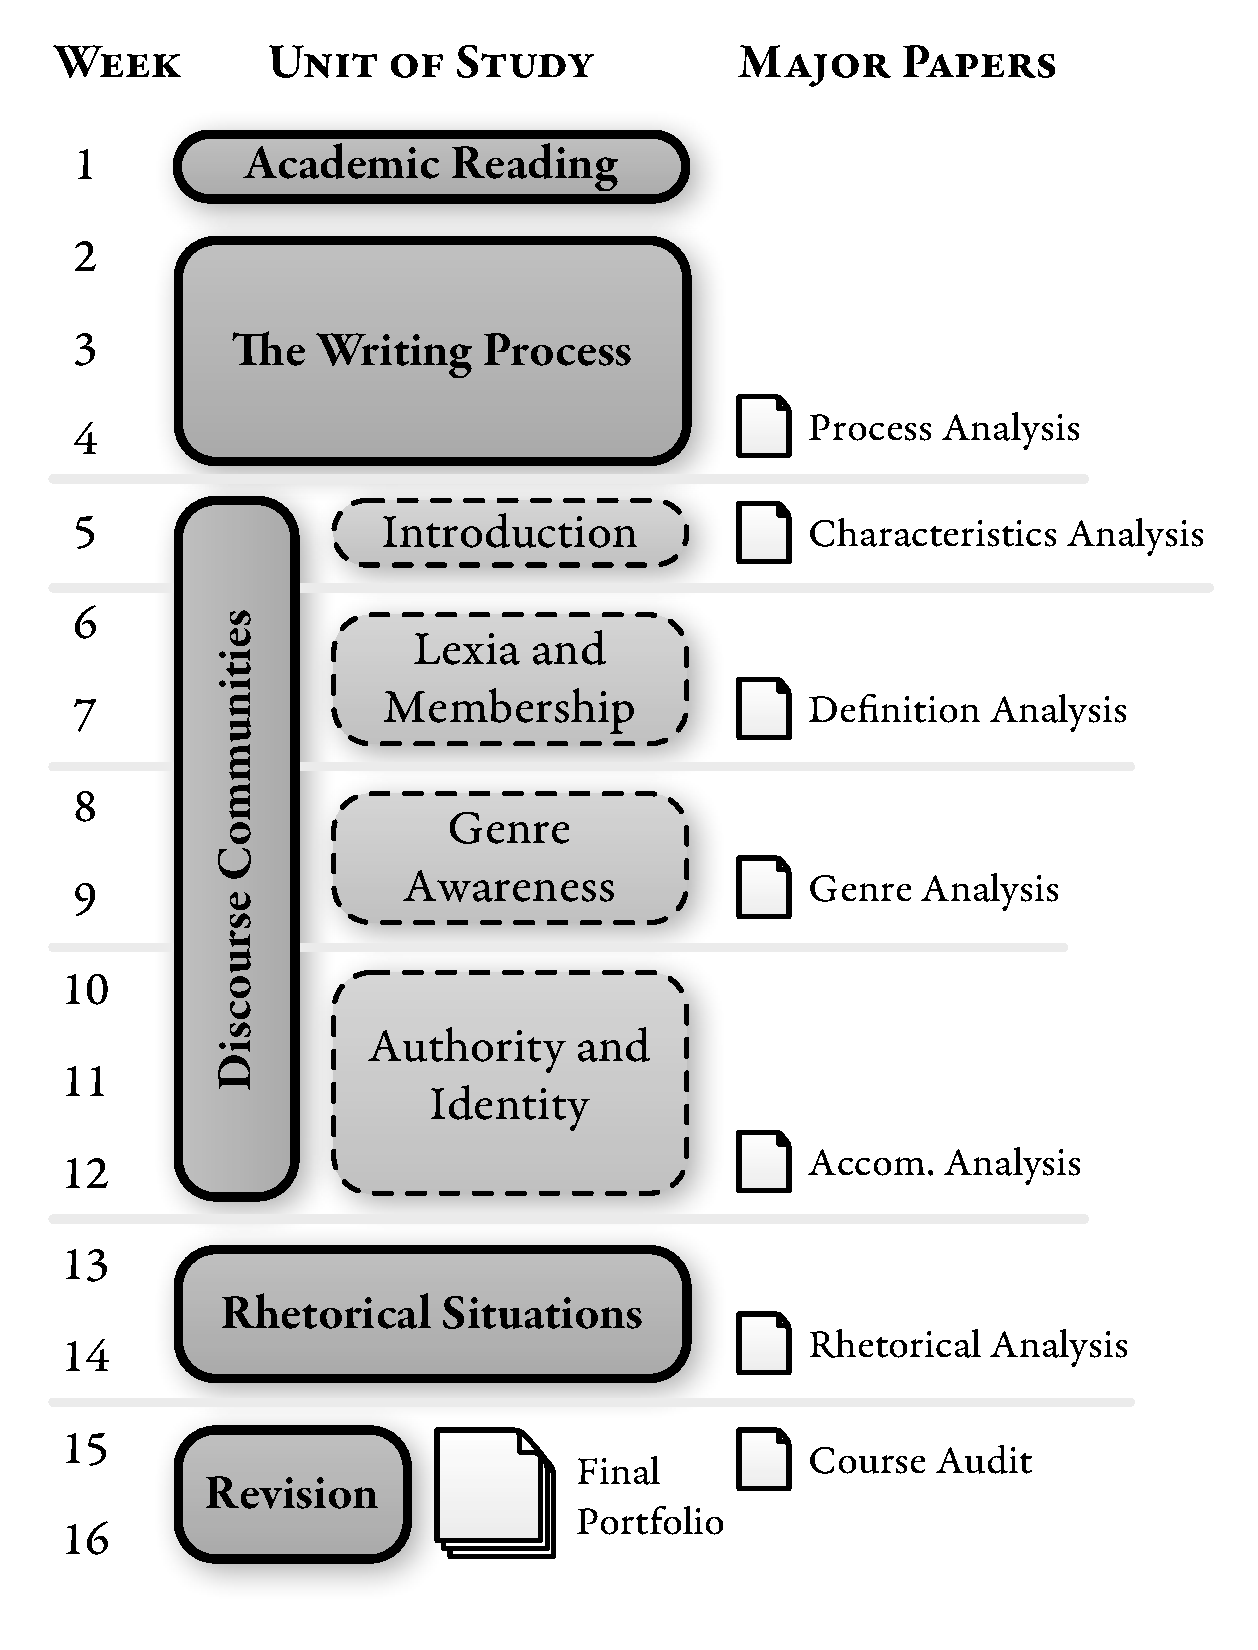
\includegraphics[width=.62\textwidth]{visual-syllabus.pdf}
				\label{fig:course-map}
		\end{figure}
\end{comment}

  

\section{Policies \& Miscellanea}
%\nocite{Curtis:2009uq,Tripp:2009kx,Wardle:2010fk} %ensures the syllabi I stole from will be in the Works Consulted list

\subsection{Participation}
Your attendance is mandatory, and your success in this course depends on your active engagement.  If you are absent more than three times, I will recommend that you drop the class; more than six times, and you risk failing the course.  If you must be absent, it is \emph{your} responsibility to complete the day’s activities and contact your peers to determine what you missed and how you need to recover. Any absence will cause you to forfeit the points for any participation or activities for those days. (Note that because major papers are collected online, absence from class will not affect the deadline or score for online submissions.)

Absences due to University-sponsored events—such as music performances, athletic competitions, debates, and some conferences—can excuse you from certain minor assignments (but not major papers). When participating in school-sponsored events, submit a Program Verification form to your instructor no later than the day you return to class. Absences due to religious holidays should be discussed with the instructor during the first week of the semester.

Please note that major assignments will be submitted online, so attendance (or lack thereof) does not affect your ability to submit work. You are still expected to turn in your work regardless of whether you are in class that day.

Treat participation in class activities (including discussions, peer review assignments, etc.) as evidence of attending to the course. I expect complete participation on all assignments from each student. We both know that the most boring classes are the ones where the instructor does all the talking. Don't let that be the case here. Share your thinking, provide your opinion, and join in the work. When in doubt, speak your mind—it's the only way your peers and your instructor will know what you're thinking, and the only way we can compliment, complement, or correct, as needed.


\subsection{Gordon Rule} % (fold)
\label{sub:gordon_rule}
\ac{1101} is a Gordon Rule class, meaning that you will be writing at least four major assignments, and you must earn a ``C'' or better to earn credit for the course. The assignments that contribute to your final portfolio meet this Gordon Rule requirement.
% subsection gordon_rule (end)



\subsection{Etiquette}
In short, the members of this class, both the instructor and the students, are expected to behave courteously and professionally in all interactions.  Under that umbrella statement, the following general guidelines should be followed in any class here at \ac{ucf}.
	\begin{description}
	\item[Tolerance] Many of our discussions will be driven by opinions and based on challenging material.  Since we are all writers, everyone in class will have personal experiences and viewpoints that can contribute meaning to the conversations.  All participants are expected to treat others with dignity and respect and are expected to refrain from insensitive comments, including racist, ageist, sexist, classist, homophobic, or other disparaging and unwarranted views.
	\item[Timeliness] Students are expected to be ready for class at its designated time just as much as you expect the instructor to dismiss class by the designated time.  Should you arrive to class late for any reason, please do so with a minimum level of disruption.  If you need to leave class early for any reason, please notify the instructor in advance and be as non-disruptive as possible when leaving.
	\item[Cellphones] As a courtesy, all cellphones should be silenced during this or any other class. Should your phone accidentally create a distraction during class, you should take action to eliminate the distraction without adding to it.
	\item[Computers] You will need to use your computer in class regularly to collaborate with others and complete your assignments. Having the discipline of shutting off distractions (such as Facebook, chat applications, etc.) improves your ability to focus and participate meaningfully.
	\item[Messages] Grammar, spelling, and punctuation reflect the formality of the situation in which they appear.  Keep in mind that emails and discussion posts you write for this class are being read by an English teacher in a composition course.  Though I don't expect discussion posts to be perfectly error-free (they're not that important), I do expect you to treat written language with respect. Complete sentences and full words (``you'' instead of ``u'') are always a good idea, even if the intended audience is your peers.
	\item[Email] As a \ac{ucf} student, you have access to a \href{http://www.outlook.com/knights.ucf.edu}{Knights Mail} account, which will be the primary method of communication for course-related announcements and information. Your instructor generally replies to messages within 24 hours Sunday through Thursday; messages sent on Fridays or Saturdays might get a delayed response.
	\end{description}
	

\subsection{Computer Reliability}\label{sub:reliability}
Save everything, and save often.  Computer problems are regular part of life, and I expect you to prepare for them rather than use them as an excuse for late work. Every semester, your instructor has students sustain a complete hard drive failure, losing all their work. Such failures are unavoidable, but losing data is not, if you plan ahead. Working backups and protection from Windows viruses are essential to avoid the most common catastrophes.  A free Dropbox account (\href{http://db.tt/mzWxY8s}{http://dropbox.com}) provides convenient and automatic backups, allows you to access your files from any networked computer in case disaster befalls yours, and preserves old versions of files so that if a file is deleted or altered, a previous copy can be restored. Regardless of the solution you choose, know how you will keep moving if your computer fails.

\subsection{Helpful Resources} % (fold)
\label{sub:helpful_resources}
\subsubsection{Writing Assistance}\label{ssub:uwc}
The \ac{uwc} provides free help for students writing papers for class.  Consultations (which can be in-person or online) can help with planning, drafting, or revising your papers.  Consider using the \ac{uwc}'s services, particularly in the early stages of planning a document.  Learn more at \href{http://uwc.ucf.edu/}{http://uwc.ucf.edu}, by calling 407-823-2197, or by visiting the first floor of \href{https://www.map.ucf.edu/locations/18/colbourn-hall/}{Colbourn Hall}.  Please note that the weeks of midterms and finals can be very busy there; you are strongly encouraged to make a reservation. A link to the \ac{uwc} appointment scheduler is available in \href{http://webcourses.instructure.com}{Webcourses}.

\subsubsection{Research Assistance} % (fold)
\label{ssub:knowledge_commons_in_the_library_}
Located halfway back on the main floor of the main campus library and online via \href{http://library.ucf.edu/Ask/}{Ask a Librarian}, the Knowledge Commons houses very smart, very helpful, and surprisingly friendly research assistants. They know more about the library and its collections than anyone else, and they love showing off what they know. They also don't like losing to a challenge. If you have trouble finding a particular resource or are stuck and need to find another direction to go with your thinking, they should be the first folks you talk to.
% subsubsection knowledge_commons_in_the_library_ (end)

\subsubsection{Additional Support Services} % (fold)
\label{ssub:other_support_services}
\begin{description}
	\item [Counseling and Psychological Services] 407-823-2811, \href{http://map.ucf.edu/locations/27/counseling-center-caps/}{\textsc{caps}} 101, \href{http://caps.sdes.ucf.edu}{http://caps.sdes.ucf.edu}
	\item [Knights Helping Knights Pantry] 407-\textsc{ucf-food}, \href{http://map.ucf.edu/locations/7g/ferrell-commons-g-fc-g/}{\textsc{fc-g}} 171, \href{http://knightspantry.org}{http://knightspantry.org}
	\item [Student Disability Services] 407-823-2371 (\textsc{tdd} 407-823-2116), \href{http://map.ucf.edu/locations/7g/ferrell-commons-g-fc-g/}{\textsc{fc-g}} 185, \href{http://sds.sdes.ucf.edu}{http://sds.sdes.ucf.edu}
	\item [Other] See the Student Development and Enrollment Services (\textsc{sdes}) site for a complete listing of offices available to assist students:  \href{http://www.sdes.ucf.edu/departments}{http://www.sdes.ucf.edu/departments}
\end{description}
% subsubsection other_support_services (end)

% subsection helpful_resources (end)

\subsection{Plagiarism}
Students at \ac{ucf} are expected to act with integrity, in terms of both classroom behavior and intellectual property.  For details, please see the \href{http://www.goldenrule.sdes.ucf.edu}{Golden Rule Student Handbook}, section \textsc{ucf}-5.008.1.e.  Violations of this ethical cornerstone will result in disciplinary action, which can include any of the following:
\begin{itemize}
	\item loss of credit on an assignment
	\item a ``Z grade'' for the course (see \href{http://z.ucf.edu}{http://z.ucf.edu} for details)
	\item loss of credit for the course
	\item removal from the University
\end{itemize}
In an effort to protect the integrity of your work and ensure it is not re-used by others later, your instructor may ask that your assignments be submitted to Turnitin.com by their deadlines.
%\todo{Am I sure? Do I want to do this? Can it be integrated with \href{http://webcourses.instructure.com}{Webcourses}?}  

In this course, we will be discussing the use of outside texts for writing in and out of the classroom, specifically the use of source documentation/citation/attribution. If you have questions about correct documentation of sources, consult a writing handbook (such as \citetitle{lunsford:2010aa} by Andrea Lunsford), the style guide for the citation system you are using (such as \citetitle{gibaldi:2009aa} by Joseph \citeauthor{gibaldi:2009aa}), the \ac{uwc} (see Section~\ref{ssub:uwc}), or your instructor during office hours. Use of outside sources without proper credit, turning in work that is not your own, or assisting others to do either are each considered plagiarism and are subject to the above consequences.

\subsection{Accommodations}
At \ac{ucf}, we are committed to providing reasonable accommodations for all persons with disabilities. Students with disabilities who need accommodations in this course must contact the instructor at the beginning of the semester to discuss needed accommodations. No accommodations will be provided until the student has 1) registered with Student Disability Services (\href{http://map.ucf.edu/locations/7g/ferrell-commons-g-fc-g/}{\textsc{fc-g}} 185, phone 407-823-2371, or \textsc{tty/tdd} 407-823-2116), and 2) met with the instructor to request accommodations.

More personally, I am dedicated to incorporating inclusive practices for all students within the classroom, as well as providing for specific accommodation requests. Beyond the provisions of Student Disability Services, please feel free to contact me with any suggestions and/or requests you have regarding the accessibility of information and/or interactions in this course. I am always interested in these types of suggestions, as they may not only meet a specific student's needs, but could be employed to make the overall class more accessible and inclusive for all students.\footnote{The second ¶ in the ``Accommodations'' section is adapted from the syllabus of Barbi Smyser-Fauble, \textsc{isu}.}

\subsection{\textsc{ucf} Allies} % (fold)
\label{sub:allies}
Your instructor is a \ac{ucf} Ally for the lesbian, gay, bisexual, transgendered, and questioning (\textsc{lgbtq}) community on campus. All \ac{ucf} Allies offer acceptance, support, and a safe space for anyone who is \textsc{lgbtq} or is working with issues of sexual identity. Allies answer questions and hold discussions in an open and non-judgmental way, and they can refer you to campus and community resources, as needed. All \ac{ucf} Allies have attended a training workshop to learn about about oppression, heterosexism, homophobia, the coming out process, and the benefits and responsibilities of being an Ally. Your instructor occasionally helps facilitate these workshops, so you are especially welcome to reach out to him to discuss any related issues. Feel free to visit during office hours or contact him by email. For more information about the \ac{ucf} Allies program, visit \href{http://allies.sdes.ucf.edu/faq}{http://allies.sdes.ucf.edu/faq}.
% subsection allies (end)

\subsection{Instructor's Research} % (fold)
\label{sub:instructor_s_research}
For the purposes of conducting research or improving his teaching practices, your instructor may use your work anonymously as an example in other classes, in workshops and lectures, or in publications. For example, I might quote from one of your assignments in a journal article or conference presentation, without revealing your identity. If you do \textbf{not} wish your work to be used in this manner, let me know in writing (via email is fine) within one week after the date your final grade is available. (This date is listed on \href{http://registrar.sdes.ucf.edu/calendar/academic/}{\ac{ucf}’s Academic Calendar}.) Your course grade will not be affected by your decision to permit or deny my use of your work. You can ensure my impartiality by notifying me after the date grades are due, which is also listed on \href{http://registrar.sdes.ucf.edu/calendar/academic/}{\ac{ucf}’s Academic Calendar}.\footnote{The ``Instructor's Research'' section is adapted from the syllabus of Beth Rapp-Young, \textsc{ucf}.}
% subsection instructor_s_research (end)

%\begin{landscape}
\clearpage%\ \newpage
%\addtocounter{page}{-2}
\section{Course Calendar}
\label{sec:calendar}
{\centering
\footnotesize %brace balanced at end of calendar
%\vspace{-1in}
\tablehead{\toprule\textbf{\textsc{Unit}} & \textbf{\textsc{Week}} & \textbf{\textsc{Date}} & \textbf{\textsc{Readings/Homework\newline(Before Class)}} & \textbf{\textsc{Guiding Question\newline(During Class)}}\\}
\tablelasthead{\toprule\textbf{\textsc{Unit}} & \textbf{\textsc{Week}} & \textbf{\textsc{Date}} & \textbf{\textsc{Readings/Homework\newline(Before Class)}} & \textbf{\textsc{Guiding Question\newline(During Class)}}\\}
\begin{mpxtabular}{>{\bfseries}p{0.75in}ccp{1.85in}p{1.85in}} % for portrait
%\begin{xtabular}{>{\bfseries}lccp{2.25in}p{3.25in}} % for landscape
%	\toprule\textbf{\textsc{Topic(s)}} & \textbf{\textsc{Week}} &\textbf{\textsc{Class Discussion}} & \textbf{\textsc{Readings/Homework}}\\

%%%%%%%%%%%%%%%%%%%%%%% Material below pasted from Numbers. Make edits there, not here.




\midrule	"Reading 
in the University"	&	1	&	6 Jan	&	n/a	&	What is a “Composition Class”?			\\
\cmidrule(l){3-5}		&		&	8 Jan	&	"Swales, “Create a Research Space (CARS)” WAW 6–8
Syllabus Quiz"	&	What are the tricks to reading a research article in an academic journal?	\newline\textbf{	\textsc{ucf} Drop/Swap Deadline Thursday	}\\
\midrule	The Writing Process	&		&	10 Jan	&	Perl, “Composing Process” WAW 191–215	&	How can we study the writing process if it’s all in our head?	\newline\textbf{	\textsc{ucf} Add Deadline	}\\
\cmidrule(l){2-5}		&	2	&	13 Jan	&	Skim EW 52–56; write self-portrait; record yourself writing it	&	What makes a person a “bad writer”?	\newline\textbf{	2-page Writer Self-Portrait Due	}\\
\cmidrule(l){3-5}		&		&	15 Jan	&	"Lamott, “Shitty First Drafts” WAW 301–304
Keep a complete writing journal for two days."	&	What makes a document or essay “bad writing”?			\\
\cmidrule(l){3-5}		&		&	17 Jan	&	"Berkenkotter and Murray, “Decisions and Revisions…” and “Response of a Lab Rat…” WAW 216–235
D/J 1, 2"	&	How can the audience influence what authors write?			\\
\cmidrule(l){2-5}		&	3	&	20 Jan	&\multicolumn{2}{c}{\textbf{	Martin Luther King, Jr. Day—No class		}}			\\
\cmidrule(l){3-5}		&		&	22 Jan	&	Transcribe your recording: How would you apply Perl’s process to it?	&	What can you look for in your transcriptions?			\\
\cmidrule(l){3-5}		&		&	24 Jan	&	Make a claim/thesis based on your coding.	&	What can you assert or conclude based on your observations?			\\
\cmidrule(l){2-5}		&	4	&	27 Jan	&	EW, 82–94 (Reviewing and Revising); review assignment sheet	&	What do we mean by “revising”? What are you qualified to review?			\\
\cmidrule(l){3-5}		&		&	29 Jan	&	Write shitty first draft of Process Analysis	&	What can other students do to make their papers as awesome as yours?			\\
\cmidrule(l){3-5}		&		&	31 Jan	&	Finalize Process Analysis	&	What have we figured out so far?	\newline\textbf{	Process Analysis Due	}\\
\midrule	Discourse Communities	&	5	&	3 Feb	&	Swales, “The Concept of Discourse Community” WAW 466–480	&	What is a Discourse Community?			\\
\cmidrule(l){3-5}		&		&	5 Feb	&	Review Characteristics assignment sheet; brainstorm groups	&	How do certain groups exhibit Swales’ characteristics?			\\
\cmidrule(l){3-5}		&		&	7 Feb	&	Brainstorm a list of new vocabulary words from this class	&	What are the effects of a community’s specific lexis?			\\
\midrule	\textmd{\emph{Lexia}}	&	6	&	10 Feb	&	Gee, “Literacy, Discourse, and Linguistics: Introduction” WAW 481–495	&	How can language control group membership?			\\
\cmidrule(l){3-5}		&		&	12 Feb	&	Choose a term with specific, rich meaning in an academic discourse; bring dictionary definition.	&	What does it mean to be “literate”?			\\
\cmidrule(l){3-5}		&		&	14 Feb	&	Find discipline-specific definition of your term.	&	What is “mushfaking”, and is it a good thing?			\\
\cmidrule(l){2-5}		&	7	&	17 Feb	&	Ask member of community how he/she learned the term	&	What are your non-dominant discourses?			\\
\cmidrule(l){3-5}		&		&	19 Feb	&	Write shitty first draft of Definition paper	&	How much can you learn about a group through the words they use?			\\
\cmidrule(l){3-5}		&		&	21 Feb	&	Identify traits/characteristics of academic articles	&	Why do we write the way(s) we do?	\newline\textbf{	Multi-Dimensional Definition Due	}\\
\midrule	\textmd{\emph{Genre}}	&	8	&	24 Feb	&	Devitt, “Generalizing about Genre” (Get from Webcourses), pp.\ 573–580	&	What “recurring situations” exist in academic writing?			\\
\cmidrule(l){3-5}		&		&	26 Feb	&	Write one message in two genres	&	What affordances and constraints are created by the genres we use?			\\
\cmidrule(l){3-5}		&		&	28 Feb	&	Porter, “Intertextuality and the Discourse Community” WAW 86–96	&	What is plagiarism?			\\
\cmidrule(l){2-5}		&	X	&	3--7 Mar	&\multicolumn{2}{c}{\textbf{	Spring Break—No class		}}			\\
\cmidrule(l){2-5}		&	9	&	10 Mar	&	Brainstorm groups that could benefit from an awareness of genre, intertextuality, or discourse communities	&	How do writers decide what genre to use for their ideas?			\\
\cmidrule(l){3-5}		&		&	12 Mar	&	Write shitty first draft of Genre Analysis	&	What can we learn about a situation by looking at the written responses to it?			\\
\cmidrule(l){3-5}		&		&	14 Mar	&	"Wardle, “Identity, Authority, and Learning to Write in New Workplaces” WAW 520–537
D/J 4, 6"	&	What could we have told Alan to make things work?	\newline\textbf{	Genre Analysis Due	}\\
\cmidrule(l){2-5}		&	10	&	17--21 Mar	&\multicolumn{2}{c}{\textbf{	Friend at Conference—No class (\textsc{ucf} Withdrawal Deadline 3/18)		}}			\\
\midrule	\textmd{\emph{Authority}}	&	11	&	24 Mar	&	"Penrose and Geisler, “Reading and Writing Without Authority” WAW 602–617
D/J 1, 2"	&	What advice do you have for Janet? for Roger?			\\
\cmidrule(l){3-5}		&		&	26 Mar	&	Read Science Accommodation sheet	&	What kind of authority can you bring to your papers? to your major?			\\
\cmidrule(l){3-5}		&		&	28 Mar	&	Mirabelli, “Learning to Serve” WAW 538–555	&	How do genre and authority relate?			\\
\cmidrule(l){2-5}		&	12	&	31 Mar	&	"McCarthy, “Stranger in Strange Lands” WAW 667–699
D/J  1, 3, 7"	&	What advice do you give to Dave? What advice does McCarthy give you?			\\
\cmidrule(l){3-5}		&		&	2 Apr	&	Bring in article on science finding	&	Which of your two articles is better? (Why is that a trick question?)			\\
\cmidrule(l){3-5}		&		&	4 Apr	&	"Keller, “Studies Explore…” WAW 595–601
D/J 1, 2"	&	How different can two articles be if they’re about the same thing?			\\
\cmidrule(l){2-5}		&	13	&	7 Apr	&	Write shitty first draft of Science Accommodation	&	How can your writing show the conversation?			\\
\cmidrule(l){3-5}		&		&	9 Apr	&	"Grant-Davie, “Rhetorical Situations and Their Constituents” in WAW textbook
D/J 1, 3, 5"	&	How can writing be a negotiation?			\\
\midrule	Rhetorical\newline Situations	&		&	11 Apr	&	"Haas and Flower, “Rhetorical Reading Strategies and the Construction of Meaning” WAW 120–38
D/J 1, 3"	&	Who are Haas and Flower writing to, and how can you tell? How does a reader construct new meaning while reading?	\newline\textbf{	Science Accommodation Due	}\\
\cmidrule(l){2-5}		&	14	&	14 Apr	&	Bring in informational textual artifact. Brainstorm controversial topics.	&	What are the rhetorical situations and exigencies of “informational” texts? What are the constraints of writing for school?			\\
\cmidrule(l){3-5}		&		&	16 Apr	&	Write shitty first draft of Navigating Sources	&	What are you good seeing that can make other students’ papers better?			\\
\cmidrule(l){3-5}		&		&	18 Apr	&	Finalize draft	&	What’s left to do?	\newline\textbf{	Navigating Sources Due	}\\
\midrule	Final\newline Portfolios	&	15	&	21 Apr	&	EW 99–101; write Course Audit cover letter; revise major papers; prepare final portfolio	&	How do your writing and revisions demonstrate that you “got” the course? Are you a Stranger in Strange Lands?			\\
\cmidrule(l){2-5}		&	16	&	Exams	&	Finalize your portfolio	&	Any last-minute panic attacks?	\newline\textbf{	Portfolio Due	}\\





%%%%%%%%%%%%%%%%%%%%%%% Material above pasted from Numbers. Make edits there, not here.
 
	\bottomrule
    \end{mpxtabular}
} %matches the \footnotesize at top of calendar
%    \end{center}

\subsection{Changes}
    Material in the preceding schedule is subject to change at the discretion of the instructor.  Students will be notified of any changes in class.  If relevant, changes will also be reflected on \href{https://webcourses.ucf.edu/webct/logon/15263651955041}{Webcourses}.

\subsection{Final Exams} % (fold)
\label{sub:final_exams}
Because this class includes a portfolio that documents your progress over the semester, there is no final exam. However, all instructors at \textsc{ucf} are required to hold class during exam periods. Therefore, for students having trouble submitting their final portfolios, a troubleshooting class will be held during the exam periods below. These class sessions will meet in the Texts \& Technology Lab, located in \textsc{cnh 207c},  
	\ifsecondclass
		\textbf{Wednesday, 23 April 2014, 10:00–12:50}
	\else % 1030 only
		\textbf{Monday, 28 April 2014, 10:00–12:50}
	\fi.
% subsection final_exams (end)
  
%    \end{landscape}


\section{Works Cited}\label{works-con}
\renewcommand\refname~{\vspace{-22pt}}

\printbibliography

\end{document}  

\section{Trash} % (fold)
\label{sec:trash}

\section{Major Assignments}
Each unit of study listed in Section~\ref{major-units} includes a major writing assignment that will be included in your final portfolio (see Figure~\ref{fig:flowchart}).  While an assignment sheet with additional details and scoring rubric will be provided later for each assignment, below is a brief overview of the expectations for each.  When preparing your response to these assignments, be sure to review the individual assignment sheets, as any revisions to the assignment will be reflected in those documents, superseding the preliminary information found here.
\begin{figure}[bp]
\centering
\includegraphics[scale=0.75]{syllabus-flowchart.pdf}
\caption{General Course Pacing with Assignments\label{fig:flowchart}}
\end{figure}

\subsection{Autoethnography}\label{process-assn} (for \ref{process-unit}, Understanding the Writing Process)
	\begin{description}
	\item[Task] Write a reflective analysis of the processes and habits used by your or someone else when performing several writing tasks in multiple situations/environments.  Present the report as an ethnographic case study to be reported on to either your peers or your instructor.
	\item[Purpose] Prove to your instructor that you can:
		\begin{enumerate}
		\item recognize various writing processes;
		\item choose an appropriate approach to this writing task, given its context and audience;
		\item present your findings in a manner appropriate to your task; and
		\item organize your response in a manner that enhances understanding.
		\end{enumerate}
	\end{description}
	
\clearpage
\subsection{Discourse Community Ethnography}\label{commty-assn} (for \ref{meaning-unit}, Discourse Communities)
	\begin{description}
	\item[Task] Write an ethnographic survey of a discourse community of your choosing.  This survey should focus on the values and goals of the community and how those are reflected in the genres and other written artifacts it produces.
	\item[Purpose] Prove to your instructor that you can:
		\begin{enumerate}
		\item correctly identify a discourse community in `real life';
		\item determine the goals, values, and characteristics of that community;
		\item analyze the writing practices of the community; and
		\item show whether---not necessarily how---the community's genres illustrate its goals.
		\end{enumerate}
	\end{description}
	
	\subsection{Analysis of Science Accommodation}\label{authority-assn} (for \ref{authority-unit}, Writing With Authority)
		\begin{description}
		\item[Task] Choose a mass-media version of a scientific report and find the corresponding original research. Write an analysis of the differences between the formats, explaining to other students the \emph{reasons} for the differences you observed.
		\item[Purpose] Prove to your instructor that you can:
			\begin{enumerate}
			\item recognize differences in the writing used in each article;
			\item make and support claims about why those differences exist;
			\item draw a conclusion about the authority needed in each article.
			\end{enumerate}
		\end{description}

\subsection{Navigating Sources That Disagree}\label{meaning-assn} (for \ref{meaning-unit}, Constructing Meaning)
	\begin{description}
	\item[Task] Write a report that analyzes three sources that disagree on a specific issue of your choosing.  Provide sufficient information about the issue that your intended audience could appropriately and knowledgeably contribute to a public debate or create an editorial column.
	\item[Purpose] Prove to your instructor that you can:
		\begin{enumerate}
		\item recognize that texts are claims as part of a conversation, rather than absolute statements of unquestionable fact; 
		\item discern issues and purposes of a variety of texts from different sources;
		\item understand the impact of rhetorical situations on writing samples;
		\item identify the intended audiences in multiple sources and determine their impact on the rhetorical situations; and
		\item present your own persuasive claim appropriately given an understanding of your own rhetorical context.
		\end{enumerate}
	\end{description}
	
\subsection{Final Portfolio}\label{portfolio}
	\begin{description}
	\item[Task] Create a showcase of your best written work produced in this course, showing both your learning as a student and your development as a writer.
	\item[Purpose] Prove to your instructor that you can:
		\begin{enumerate}
		\item improve your writing style and and quality over the course of a semester;
		\item implement revision strategies on previous work; and
		\item reflect on the changes in your thinking during the term%; and
%		\item pridefully produce a professional printed product.
		\end{enumerate}
	\end{description}



\subsubsection{From DWR} % (fold)
\label{ssub:from_dwr}
In ENC1101, students read research findings from Writing Studies intended to help them gain both procedural and declarative knowledge about writing that they can generalize ("transfer") to later writing situations. Course topics include:
\begin{itemize}
	\item How writers and readers construct texts
	\item Effective writing processes and practices
	\item How discourse communities shape writing
	\item Understanding writing in the university
\end{itemize}
As students study each of these topics, they engage in writing-to-learn activities to help them understand and apply the various concepts; they also compose and revise extended texts employing those concepts at the end of each unit.
% subsubsection from_dwr (end)


\subsection{Objectives} % (fold)
\label{sub:objectives}
Through successful completion of each component of this course, you should be able to:
\begin{enumerate}
\item distinguish between heuristics and algorithms, recognizing which are appropriate systems for `rules' of writing;
\item acquire and use strategies for reading complex, college-level texts;
\item develop and effectively use an appropriate discipline-specific vocabulary to discuss writers, writing situations, and the writing process;
\item understand the concept of \emph{rhetorical situation} and be aware of its influence on your reading and writing activities, both in and out of class;
\item understand the fluid nature of the writing process through its various components and be able to apply those components conscientiously when producing written materials in various rhetorical situations;
\item understand the concepts of \emph{discourse conventions} and \emph{genres} and understand why both can differ across groups (especially groups within academia);
\item identify characteristics of a discourse community and respond to them appropriately; and
\item approach future writing situations conscientiously, using the tools listed above to make informed decisions and plans for writing tasks both in and out of school.
\end{enumerate}
% subsection objectives (end)



\begin{comment} % This entire list commented out because it provided way too much detail on schedule but not enough explanation of intent.
\setcounter{subsection}{-1}
\newcounter{week}\addtocounter{week}{1}

\subsection{Learning to read material in this course}
	\begin{itemize}
	\item Week \arabic{week}\addtocounter{week}{1}
	\item Readings
		\begin{enumerate}
		\item Introduction from \citeauthor{downs:2010aa}, \citetitle{downs:2010aa}
		\item The \textsc{cars} model, in \citeauthor{swales:1990aa}, \citetitle{swales:1990aa}
		\end{enumerate}
	\end{itemize}

\subsection {Learning how to use what other people write} (aka ``Constructing Meaning Through Texts'')
	\begin{itemize}
	\item Weeks \arabic{week}\addtocounter{week}{4}--\arabic{week}\addtocounter{week}{1}
	\item Readings
		\begin{enumerate}
		\item Brief plagiarism discussion: How \emph{not} to use what other people write
		\item \citeauthor{hass1988rhetorical}, \citetitle{hass1988rhetorical}
			\begin{description}
			\item[Homework] D\&J 2, 4
			\item[Discussion] D\&J 6, A\&E 2, 3
			\end{description}
		\item \citeauthor{grant1997rhetorical}, \citetitle{grant1997rhetorical} [2 Weeks]
			\begin{description}
			\item[Homework] D\&J 1, 2, 4
			\item[Discussion] D\&J 3, 7, 9; A\&E 2, 3 (A\&E 3 begins unit project)
			\end{description}
		\item \citeauthor{porter1986intertextuality}, \citetitle{porter1986intertextuality}
			\begin{description}
			\item[Homework] \textcolor{red}{Not in textbook yet}
			\item[Discussion] \textcolor{red}{Not in textbook yet}
			\end{description}
		\end{enumerate}
	\item Major Assignment: Navigating Sources That Disagree
	\end{itemize}

\subsection {Learning how \emph{you} write} (aka ``Understanding the Writing Process'')
	\begin{itemize}
	\item Weeks \arabic{week}\addtocounter{week}{3}--\arabic{week}\addtocounter{week}{1}
	\item Readings
		\begin{enumerate}
		\item \citeauthor{perl1979composing}, \citetitle{perl1979composing} \textbf{and} \citeauthor{lamott-shitty}, \citetitle{lamott-shitty}
			\begin{description}
			\item[Homework] D\&J 1, 7; A\&E 1
			\item[Discussion] A\&E 2; Tony and Lamott
			\end{description}
		\item \citeauthor{berkenkotter1983decisions}, \citetitle{berkenkotter1983decisions} \textbf{and} \citeauthor{haruf:2002aa}, \citetitle{haruf:2002aa}
			\begin{description}
			\item[Homework] D\&J 1, 2
			\item[Discussion] A\&E 1, 3; Haruf/Murray Comparison
			\end{description}
		\item \citeauthor{rose1980rigid}, \citetitle{rose1980rigid} \textbf{and} \citeauthor{king-writing}, \citetitle{king-writing}
			\begin{description}
			\item[Homework] D\&J 1, 2
			\item[Discussion] A\&E 1, 3
			\end{description}
		\end{enumerate}
	\item Major Assignment: Portrait of a Writer
	\end{itemize}

\subsection {Learning how to `fit in' when writing} (aka ``Discovering Discourse Communities'')
	\begin{itemize}
	\item Weeks \arabic{week}\addtocounter{week}{4}--\arabic{week}\addtocounter{week}{1}
	\item Readings
		\begin{enumerate}
		\item \citeauthor{swales:1990aa}, \citetitle{swales:1990aa}
			\begin{description}
			\item[Homework] D\&J 1, 2 (also begin research for unit project)
			\item[Discussion] D\&J 3--6
			\end{description}
		\item \citeauthor{harris1989idea}, \citetitle{harris1989idea}
			\begin{description}
			\item[Homework] D\&J 3; A\&E 1
			\item[Discussion] D\&J 1, 2, 4; A\&E 2
			\end{description}
		\item \citeauthor{penrose1994reading}, \citetitle{penrose1994reading}
			\begin{description}
			\item[Homework] D\&J 1, 2
			\item[Discussion] D\&J 3, 4; A\&E 1
			\end{description}
		\item \citeauthor{mccarthy1987stranger}, \citetitle{mccarthy1987stranger} \textbf{and} \citeauthor{hyland2000disciplinary}, Handout from \citetitle{hyland2000disciplinary}
			\begin{description}
			\item[Homework] McCarthy D\&J 2, 3, 5
			\item[Discussion] Hyland D\&J 1, 2; A\&E 1, 3, 4
			\end{description}
		\end{enumerate}
	\item Major Assignment: Discourse Community Ethnography
	\end{itemize}
\end{comment} % Removal of list without justification




\begin{comment} %Early table test for calendar
\noindent\begin{tabulary}{\textwidth}{cLLL}
	\toprule\setcounter{week}{1}
	\textbf{\textsc{Week}} & \textbf{\textsc{Topic(s)}} & \textbf{\textsc{Class Discussion}} & \textbf{\textsc{Homework}}\\
	\midrule\arabic{week}\addtocounter{week}{1} 
	& % Topic:
Reading for College
	& % Discussion:
Course Introduction; Portfolio; Swales' \textsc{cars} model
	& % Homework:
Read Introduction in text
	\\
	\bottomrule
\end{tabulary}
\end{comment} %Early test


\begin{comment} % templates for table

% New Unit
	\midrule% Topic:
UNIT
	& \arabic{week}\addtocounter{week}{1} 
	& % Discussion:
DISCUSSION
	& % Homework:
HOMEWORK
	\\

% Continued Unit
	\cmidrule(l){2-4}% Topic:
	& \arabic{week}\addtocounter{week}{1} 
	& % Discussion:
DISCUSSION
	& % Homework:
HOMEWORK
	\\

\end{comment}
